\documentclass[UTF8]{book}
\usepackage{ctex}
\usepackage[colorlinks=true]{hyperref}
\usepackage{amsmath}
\usepackage{amssymb}
\usepackage{tikz}
\usepackage{graphicx}
\usepackage{float}
\usepackage{geometry}
\usepackage{fancyhdr}
\usepackage{caption}
\usepackage{subcaption}
\usepackage[T1]{fontenc}
\usepackage{palatino}
\usepackage{booktabs}
\usepackage[stable]{footmisc}

\geometry{a4paper, left=2.5cm, top=2.5cm, bottom=2cm}
\geometry{hcentering}

\pagestyle{fancy}
\cfoot{\thepage}

\begin{document}
\title{深度学习笔记}
\author{zhliangqi}
\date{\today}

\maketitle

\tableofcontents

\chapter{Linear Algebra}

\section{Norm}
\[
    \|\vx\|_p = \biggl(\sum_i |x_i|^p\biggr)^{\frac{1}{p}}, p \in \R\ and\ p \geqslant 1
\]

范数是满足以下性质的任意函数:
\begin{itemize}
    \item $f(\vx) = 0 \Rightarrow \vx = 0$
    \item $f(\vx + \vy) \leqslant f(\vx) + f(\vy)$
    \item $\forall \alpha \in \R, f(\alpha \vx) = |\alpha|f(\vx)$
\end{itemize}

\section{Eigenvalues and Eigenvectors}
\begin{equation}
    Au = \lambda u
\end{equation}
特征值$\lambda$代表线性变化的伸缩倍数,特征向量$u$代表变换的方向

\section{Singular value decomposition}
\textbf{定义} 对于$A \in C^{m \times n}$,$rank(A) = r$,矩阵$A^HA$的特征值为
$\lambda_1 \geqslant \lambda_2 \geqslant ... \geqslant \lambda_r > 0$,
$\lambda_{r+1} = \lambda_{r+2} = ... = \lambda_{n} = 0$,称正数$\sigma_i = \sqrt{\lambda_i}(i = 1,2,...,r) $
为矩阵$A$的\textbf{奇异值}
\\
\begin{equation}
    \begin{split}
        A
        &= U \Sigma V^H \\
        &=
        \begin{pmatrix}
            u_1 & u_2 & \cdots & u_m
        \end{pmatrix}
        \left(
            \begin{array}{cccc:c}
                \sigma_1&           &           &           & \\
                        & \sigma_2  &           &           & 0\\
                        &           & \ddots    &           & \\
                        &           &           & \sigma_r  & \\
                        \hdashline
                        &           & 0         &           & 0
            \end{array}
        \right)
        \begin{pmatrix}
            v_1^H \\
            v_2^H \\
            \cdots \\
            v_n^H
        \end{pmatrix} \\
        &= \sigma_1 \boldsymbol{u}_1 \boldsymbol{v}_1^H + \sigma_2 \boldsymbol{u}_2 \boldsymbol{v}_1^H + \cdot\cdot\cdot + \sigma_r \boldsymbol{u}_r \boldsymbol{v}_r^H
    \end{split}
\end{equation}

\subsection{Dimensionality Reduction}
将图片作为矩阵进行奇异值分解,提取前n个奇异值,则可以达到图像压缩的目的.


\subsection{Matrix}
\href{https://math.stackexchange.com/questions/42649/why-are-invertible-matrices-called-non-singular}{Why are invertible matrices called 'non-singular'?}

If you take an $n \times n$ matrix "at random", then it will almost certainly be invertible. 
That is, the generic case is that of an invertible matrix, the special case is that of a matrix that is not invertible.

For example, a $1 \times 1$ matrix(with real coefficients) is invertible if and only if it is not the $\mathbf{0}$ matrix; 
for $2 \times 2$ matrices, it is invertible if and only if the two rows do not lie in the same line through the origin; 
for $3 \times 3$, if and only if the three rows do not lie in the same plane through the origin; etc.

So here, "singular" is not being taken in the sense of "single", but rather in the sense of "special", "not common". 
See the dictionary definition: it includes "odd", "exceptional", "unusual", "peculiar".

The noninvertible case is the "special", "uncommon" case for matrices. 
It is also "singular" in the sense of being the "troublesome" case (you probably know by now that when you are working with matrices, the invertible case is usually the easy one).

\textbf{满秩矩阵一定是可逆矩阵}
\chapter{statistics}

\section{期望}
\section{方差}
均匀分布$X \sim R(a, b)$
其期望为
\begin{equation}
    \begin{split}
        E(X) &= \int_{a}^{b}x f(x) \mathrm{d}x		\\
        &= \frac{1}{b-a}\int_{a}^{b}x\mathrm{d}x	\\
        &= \frac{1}{b-a} \frac{1}{2} (b^2 - a^2)	\\
        &= \frac{1}{2}(b + a)
    \end{split}
\end{equation}
其方差为
\begin{equation}
    \begin{split}
        Var(X) &= E(X - EX)^2  \\
        &= E(X)^2 - (EX)^2 \\
        &= \int_{a}^{b} x^2 f(x) \mathrm{d}x - (EX)^2 \\
        &= \frac{1}{3(b-a)} (b^3 - a^3) - \frac{1}{4}(b+a)^2 \\
        &= \frac{1}{12}(b-a)^2
    \end{split}
\end{equation}
\\
对于正态分布$N(\mu, \sigma ^2)$,其期望$E(X) = \mu$,方差为$Var(X) = \sigma^2$.

\chapter{basic}

\section{Mechine Learning}
\begin{itemize}
    \item supervised learning
    \item semi-supervised learning
    \item unsupervised learning
    \item reinforcement learning
    \item active learning
\end{itemize}

\section{iid}

\section{最小方差无偏估计}

\section{Maximum likelihood estimation}
深度学习来就是用模型$p_{model}(\boldsymbol{x};\boldsymbol{\theta})$来估计数据的真实分布$p_{data}(\boldsymbol{x};\boldsymbol{\theta})$,
对于一组确定的数据集$X$,在样本已被观察到的情况下,需要找到使得$p_{model}(X; \boldsymbol{\theta})$出现可能性最大的一组参数$\boldsymbol{\theta}$,也就是
最大似然估计:
\begin{equation}
    \begin{split}
        \boldsymbol{\theta}_{ML} &= \arg \max_\theta p_{model}(X, \boldsymbol{\theta}) \\
        &= \arg \max_{\boldsymbol{\theta}} \prod _{i=1}^m p_{model}(\boldsymbol{x}^i; \boldsymbol{\theta})
    \end{split}
\end{equation}
等价于
\begin{equation}
    \begin{split}
        \boldsymbol{\theta}_{ML} &= \arg \max_{\boldsymbol{\theta}} \sum_{i=0}^m \log p_{model}(\boldsymbol{x}^i; \boldsymbol{\theta})
    \end{split}
\end{equation}
除$m$,等价于
\begin{equation}
    \begin{split}
        \boldsymbol{\theta}_{ML} &= \arg \max_{\boldsymbol{\theta}} E _{x \sim \hat p_{data}} \log p_{model}(\boldsymbol{x}^i; \boldsymbol{\theta})
    \end{split}
\end{equation}

\subsection{KL divergence}
KL散度用来衡量两种分布之间的差异,
\begin{equation}
    \begin{split}
        D_{KL}(\hat p_{data}|| p_{model}) &= \int_{-\infty}^{+\infty} \hat p_{data}(\boldsymbol{x}) \ln{\frac{\hat p_{data}(\boldsymbol{x})}{p_{model}(\boldsymbol{x})}} \mathrm{d}x
    \end{split}
\end{equation}
$\hat p_{data}(\boldsymbol{x})$与模型无关

\section{Initialization scheme}
\subsection{constant initialization}

\subsection{random initialization}
按照某一分布随机初始化
\subsubsection{normal initialization}
\begin{equation}
    W \sim N(\mu, \sigma^2)
\end{equation}

\subsubsection{uniform initalization}
\begin{equation}
    W \sim U[-\frac{1}{\sqrt{n}}, \frac{1}{\sqrt{n}}]
\end{equation}

\subsection{xavier initalization}
针对使用\textbf{对称激活函数}$\tanh(x)$的网络进行参数初始化,对于ReLU激活函数并不适用\cite{Glorot2010}.

\subsubsection{Forward}
对于一个卷积层来说
\begin{equation}
    \begin{split}
        \mathbf{y}_l &= \mathbf{W}_l \mathbf{x}_l + \mathbf{b}_l\\
        \mathbf{x}_l &= f(\mathbf{y}_{l-1})
    \end{split}
\end{equation}
在如下前提和假设下
\begin{itemize}
    \item 初始化$\mathbf{W}_l$元素为独立同分布
    \item 假设$\mathbf{x}_l$元素也为独立同分布
    \item $\mathbf{w}_l$, $\mathbf{x}_l$互相独立
\end{itemize}
则有
\begin{equation}
    \begin{split}
        Var(\mathbf{y}_l) &= Var(\sum \mathbf{w}_l \mathbf{x}_l + \mathbf{b}_l)\\
        &= Var(\sum \mathbf{w}_l \mathbf{x}_l) \\
        &= n_l Var(\mathbf{w}_l \mathbf{x}_l)
    \end{split}
\end{equation}
令$\mathbf{w}_l$期望为0,$E(\mathbf{w}_l) = 0, Var(\mathbf{w}_l) = E(\mathbf{w}_l - E(\mathbf{w}_l))^2 = E\mathbf{w}_l^2$,则
\begin{equation}
    \begin{split}
        Var(\mathbf{y}_l) &= n_l E(\mathbf{w}_l^2\mathbf{x}_l^2) - n_l E^2\mathbf{w}_l E^2 \mathbf{x}_l \\
        &= n_l E(\mathbf{w}_l^2\mathbf{x}_l^2) \\
        &= n_l Var(\mathbf{w}_l)E(\mathbf{x}_l^2)
    \end{split}
\end{equation}
若$E\mathbf{x}_l = 0$,则
\begin{equation}
    Var(\mathbf{y}_l) = n_l Var(\mathbf{w}_l)Var(\mathbf{x}_l)
\end{equation}

若要实现$Var(\mathbf{y}_l) = Var(\mathbf{x}_l)$,则需要满足$n_l Var(\mathbf{w}_l) = 1$,即
\begin{equation}
    Var(\mathbf{w}_l) = \frac{1}{n_l}
\end{equation}

\begin{itemize}
    \item 若$\mathbf{w}_l$服从正态分布,则$\mathbf{w}_l \sim N(0, \frac{1}{n_l})$
    \item 若$\mathbf{w}_l$服从均匀分布,则$\mathbf{w}_l \sim U(-\sqrt{\frac{3}{n_l}}, \sqrt{\frac{3}{n_l}})$
\end{itemize}

\subsubsection{Backword}
反向传播过程中,需要保证梯度的方差不变,每一层的梯度为:
\begin{equation}
    \Delta \mathbf{x}_l = \hat{\mathbf{W}}_l \Delta \mathbf{y}_l
\end{equation}
假设
\begin{itemize}
    \item $\mathbf{w}_l$和$\Delta{\mathbf{y}}_l$互相独立
    \item $E\mathbf{w}_l = 0, E\Delta{\mathbf{x}}_l = 0$
\end{itemize}
同前向传播,可得
\begin{equation}
    \begin{split}
        Var(\Delta{\mathbf{x}_l}) &= \hat n_l Var(\mathbf{w}_l)Var(\Delta{\mathbf{y}}_l)
    \end{split}
\end{equation}
\begin{itemize}
    \item 若$\mathbf{w}_l$服从正态分布, 则$\mathbf{w}_l \sim N(0, \frac{1}{\hat n_l})$
    \item 若$\mathbf{w}_l$服从均匀分布,则$\mathbf{w}_l \sim U(-\sqrt{\frac{3}{\hat n_l}}, \sqrt{\frac{3}{\hat n_l}})$
\end{itemize}

除非$n = \hat n_l$,否则同时保证信号在向前向后传播时的Var不变,取调和平均数,$Var(\mathbf{w}_l) = \frac{2}{n_l + \hat n_l}$,可得
\begin{itemize}
    \item Normal distribution: $\mathbf{w}_l \sim N(0, \frac{2}{n_l + \hat n_l})$
    \item Uniform distribution: $\mathbf{w}_l \sim U(-\sqrt{\frac{6}{n_l+\hat n_l}}, \sqrt{\frac{6}{n_l+\hat n_l}})$
\end{itemize}


\subsection{orthogonal initalization}

\subsection{kaiming initalization}
Xavier 针对对称激活函数的层权重初始化进行设计,但对于使用ReLu激活函数的层并不适用。\\
对ReLU层来说,$E(\mathbf{x}_l^2) = \frac{1}{2}Var(\mathbf{y}_l)$,因此
\begin{equation}
    \begin{split}
        Var(\mathbf{y}_l) &= \frac{1}{2} n_l Var(\mathbf{w}_l)Var(\mathbf{x}_l) \\
        Var(\Delta{\mathbf{x}_l}) &= \frac{1}{2} \hat n_l Var(\mathbf{w}_l)Var(\Delta{\mathbf{y}}_l)
    \end{split}
\end{equation}
且在权重初始化时,使用上述任意一个即可。

\section{正则化}

\section{Data proprocessing}
\subsection{whitening}

\section{Activation functions}
\subsection{sigmoid}
\begin{tikzpicture}[domain=-2:2]
    \draw[very thin,color=gray] (-1.9, -1.9) grid (1.9, 1.9);
    \draw[->] (-2,0) -- (2,0) node[right] {$x$};
    \draw[->] (0,-2) -- (0,2) node[above] {$f(x)$};
    \draw[color=red]	plot (\x, { 1 / (1 + exp(-\x)) })   	node[right] {$g(x) = \frac{1}{1 + \mathrm{e^{-x}}}$};
\end{tikzpicture}

\begin{equation}
    \begin{split}
        g(x) &= \frac{1}{1+\mathrm{e}^{-x}} \\
        g(x)' &= g(x)(1-g(x))
    \end{split}
\end{equation}

\subsection{tanh(x)}
\begin{tikzpicture}[domain=-2:2]
    \draw[very thin,color=gray] (-1.9, -1.9) grid (1.9, 1.9);
    \draw[->] (-2,0) -- (2,0) node[right] {$x$};
    \draw[->] (0,-2) -- (0,2) node[above] {$f(x)$};
    \draw[color=blue]	plot (\x,{tanh(\x)})					node[right] {$g(x) = \tanh(x)$};
\end{tikzpicture}

\begin{equation}
    \begin{split}
        g(x) &= tanh(x) \\
        g(x)' &= 1 - g(x)^2 \\ &= 1 - \tanh(x)^2
    \end{split}
\end{equation}

\subsection{Rectified linear units}
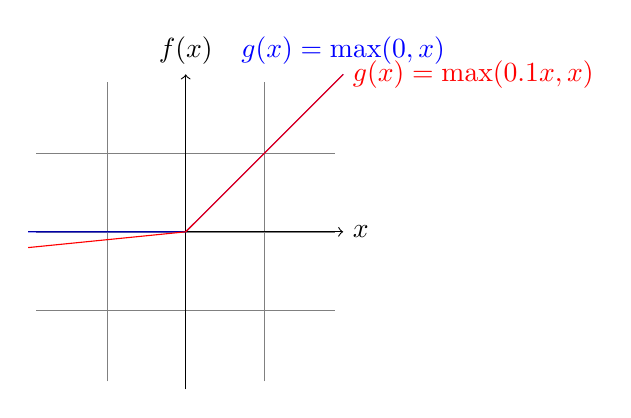
\begin{tikzpicture}[domain=-2:2]
    \draw[very thin,color=gray] (-1.9, -1.9) grid (1.9, 1.9);
    \draw[->] (-2,0) -- (2,0) node[right] {$x$};
    \draw[->] (0,-2) -- (0,2) node[above] {$f(x)$};
    \draw[color=blue]	plot (\x,{max(0, \x)})					node[above] {$g(x) = \max(0, x)$};
    \draw[color=red]	plot (\x,{max(0.1 * \x, \x)})			node[right] {$g(x) = \max(0.1x, x)$};
\end{tikzpicture}

\subsubsection{ReLU}
\begin{equation}
    g(x) = \max(0, x)
\end{equation}

\subsubsection{Leaky ReLU}
\begin{equation}
    g(x) = \max(0.01x, x)
\end{equation}

\subsubsection{PReLU}
\begin{equation}
    g(x) = \max(\alpha x, x)
\end{equation}

\subsection{haha}
\begin{tikzpicture}[domain=-2:2]
    \draw[very thin,color=gray] (-1.9, -1.9) grid (1.9, 1.9);
    \draw[->] (-2,0) -- (2,0) node[right] {$x$};
    \draw[->] (0,-2) -- (0,2) node[above] {$f(x)$};
    \draw[color=blue]	plot (\x,{tanh(\x) + 0.25 * \x})					node[right] {$g(x) = \tanh(x) + 0.25x$};
\end{tikzpicture}

\begin{equation}
    \begin{split}
        g(x) &= \tanh(x) + 0.25x \\
        g(x)' &= 0.75 - g(x)^2 \\ &= 0.75 - \tanh(x)^2
    \end{split}
\end{equation}

\subsection{Loss functions}


\chapter{Optimization Algorithms}
如果梯度只用来指示方向,大小完全由lr决定?
\section{Challenges}

\begin{figure}
    \centering
    \begin{minipage}[b]{0.32\textwidth}
        \centering
        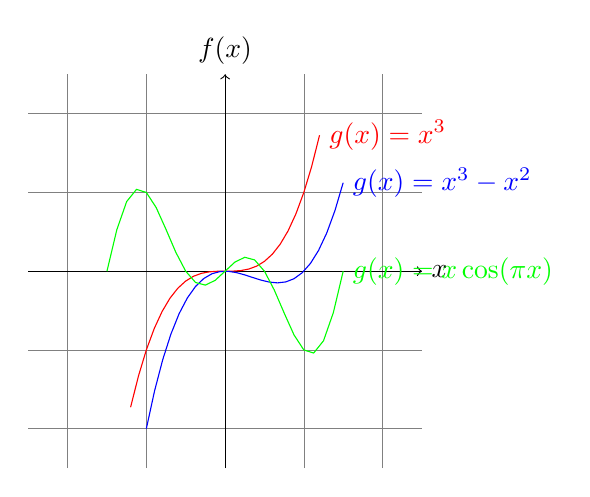
\begin{tikzpicture}
            \draw[very thin,color=gray] (-2.5, -2.5) grid (2.5, 2.5);
            \draw[->] (-2.5,0) -- (2.5,0) node[right] {$x$};
            \draw[->] (0,-2.5) -- (0,2.5) node[above] {$f(x)$};
            \draw[red,domain=-1.2:1.2]	plot (\x, { \x * \x * \x })   	node[right] {$g(x) = x^3 $};
            \draw[blue,domain=-1.0:1.5]	plot (\x, { \x * \x * \x - \x * \x })   	node[right] {$g(x) = x^3 - x^2$};
            \draw[green,domain=-1.5:1.5]	plot (\x, { \x * cos(3.1415926 * \x r) })   	node[right] {$g(x) = x\cos(\pi x) $};
        \end{tikzpicture}
    \end{minipage}
    \begin{minipage}[b]{0.32\textwidth}
        \centering
        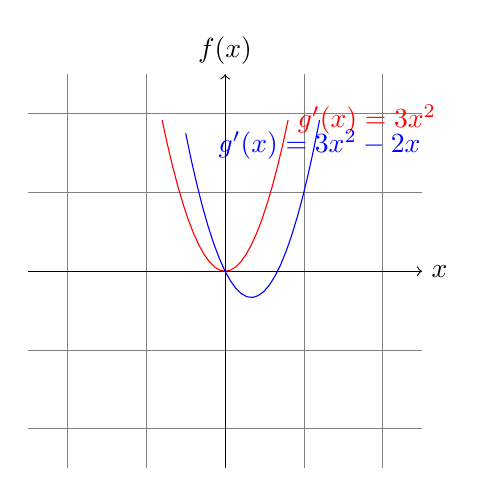
\begin{tikzpicture}
            \draw[very thin,color=gray] (-2.5, -2.5) grid (2.5, 2.5);
            \draw[->] (-2.5,0) -- (2.5,0) node[right] {$x$};
            \draw[->] (0,-2.5) -- (0,2.5) node[above] {$f(x)$};
            \draw[red,domain=-0.8:0.8]	plot (\x, { 3 * \x * \x })   	node[right] {$g'(x) = 3x^2 $};
            \draw[blue,domain=-0.5:1.2]	plot (\x, { 3 * \x * \x - 2 * \x})   	node[below] {$g'(x) = 3x^2 - 2x$};
        \end{tikzpicture}
    \end{minipage}
    \begin{minipage}[b]{0.32\textwidth}
        \centering
        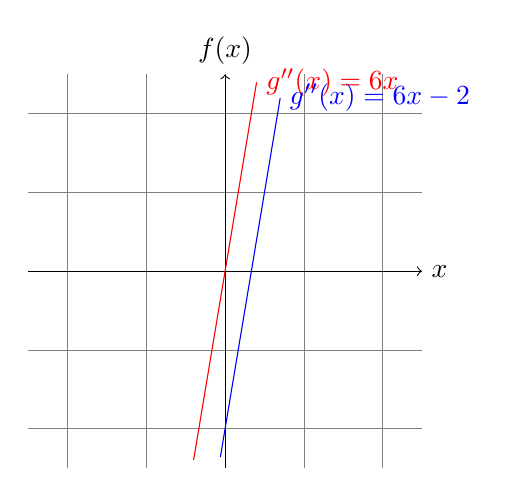
\begin{tikzpicture}
            \draw[very thin,color=gray] (-2.5, -2.5) grid (2.5, 2.5);
            \draw[->] (-2.5,0) -- (2.5,0) node[right] {$x$};
            \draw[->] (0,-2.5) -- (0,2.5) node[above] {$f(x)$};
            \draw[red,domain=-0.4:0.4]	plot (\x, { 6 * \x })   	node[right] {$g''(x) = 6x $};
            \draw[blue,domain=-0.06:0.7]	plot (\x, { 6 * \x - 2 })   	node[right] {$g''(x) = 6x - 2$};
        \end{tikzpicture}
    \end{minipage}
    \caption{Challenges}
\end{figure}


\subsection{Local Minima}
\begin{quotation}
    When the numerical solution of an optimization problem is near the local optimum, the numerical
    solution obtained by the final iteration may only minimize the objective function locally, rather
    than globally, as the gradient of the objective function's solutions approaches or becomes zero.
    \textit{Only some degree of noise might knock the parameter out of the local minimium. In fact,
        this is the one of the beneficial properties of stochastic gradient descent where the natural variation
        of gradients over minibatches is able to dislodge the parameters from loacl minima.}\cite{zhang2020dive}
\end{quotation}
\subsection{Saddle Points}
\begin{quotation}
    We assume that the input of a function is $k$-dimensional vector and its ouput is a scalar,
    so its \textit{Hession matrix} will have \textit{$k$ eigenvalues}. The solution of the function could
    be a local minimum, a local maximum or a saddle point at a position where the function gradient
    is zero:
    \begin{itemize}
        \item When the eigenvalues of the function's Hession matrix at the zero-gradient position 
        are all positive, we have a local minimum for the function.
        \item When the eigenvalues of the function's Hession matrix at the zero-gradient position 
        are all negative, we have a local maximum for the function.
        \item When the eigenvalues of the function's Hession matrix at the zero-gradient position 
        are negative and positive, we have a saddle point for the function.
        \item 同号且至少有一个为0,不确定
    \end{itemize}
    For high-dimensional problem the likehood that at least some of the eigenvalues are negative
    is quite high. This makes sadlle points are more likely then local minima.\cite{zhang2020dive}
\end{quotation}

\subsection{Vanishing gradients}
\begin{quotation}
    Vanishing gradients can cause optimization to stall. Often a reparameterization of the problem
     helps. Good initialization of the parameters can be beneficial, too.\cite{zhang2020dive}
\end{quotation}

\subsection{Gradient Descent}
Using a Taylor expansion we obtain that:
\begin{equation}
    f(x + \epsilon) = f(x) + \epsilon f'(x) + \mathcal{O} (\epsilon^2)
\end{equation}
\par
For small $\epsilon$ moving in \textit{the direction of negative gradient} will decrease $f$. Choose $\epsilon = 
-\eta f'(x), \eta > 0$, then we get:
\begin{equation}
    f(x - \eta f'(x)) = f(x) - \eta f'^2(x) + \mathcal{O} ((\eta f'(x))^2)
\end{equation}
\par Choose $\eta$ samll enough for the higher order terms to become irrelevant. then
\begin{equation}
    f(x - \eta f'(x)) \lessapprox f(x)
\end{equation}
that means, if we use 
\begin{equation}
    x \leftarrow x - \eta f'(x)
\end{equation}
to iterate x, the value of $f(x)$ decline.

\subsection{Adaptive Methods}
Getting the learning rate 'just right' is tricky. What if we could determine $\eta$ automatically or get rid of having to select
a setp size at all? Second order methods that look not only at the value and gradient of the objective but alse at its \textit{curvature}
can help in this case. These methods cannot be applied to deep learning directly due to the computational cost.

\subsubsection{Newton's Method}
当Taylor expansion展开到二阶导数时:
\begin{equation}
    f(\mathbf{x} + \epsilon) = f(\mathbf{x}) + \epsilon^\top \nabla f(\mathbf{x}) + \frac{1}{2} \epsilon^\top H_f \epsilon 
    + \mathcal{O}(\|\epsilon\|^3)
\end{equation}
we define $H_f := \nabla \nabla ^\top f(\mathbf{x})$ to be the \textit{Hession} of $f$. $H$ is a $d \times  d$ matrix and may be
prohibitively large, due to the cost of storing $\mathcal{O}(d^2)$ entries.

\par

After all, the minimum of $f$ statifies $\nabla f(\mathbf{x}) = 0$.  Taking derivatives of above equtaion with regard to $\eta$ and 
ignoring higher order terms we arrive at 
\begin{equation}
   \begin{split}
    \nabla f(\mathbf{x}) + H_f \epsilon = 0 \\
    \mathbf{\epsilon} = -H_f^{-1} \nabla f(\mathbf{x})
   \end{split}
\end{equation}

then, $\epsilon = -\eta \nabla f(\mathbf{x})$, we get
\begin{equation}
    \begin{split}
        \mathbf{\eta} = -H_f^{-1}
    \end{split}
\end{equation}

For $f(x) = (x-2)(x-4) = x^2 - 6x + 8, f'(x) = 2x - 6, f''(x) = 2$, then
\begin{equation}
    \epsilon = -f''(0)^{-1} f'(0) = -\frac{1}{2} \times -6 = 3 
\end{equation}

\subsubsection{Hessian}
Hession 矩阵是是对称的,可以表示为一组特征值和一组特征向量的正交基底,在特定方向上$g$上的二阶导数为$g^\top H g$,当$g$为特征向量时,这个二阶导数就是
对应的特征值。最大特征值确定最大二阶导数,最小特征值确定最小导数。\par
在$g$方向上的learning rate为
\begin{equation}
    \eta_g = \frac{1}{g^\top H_f g}
\end{equation}
最差的情况下,$g$与$H$最大的特征值$\lambda_{max}$对应的特征向量对齐,此时的最优步长为$\frac{1}{\lambda_{max}}$,当要最小化的目标函数能用二次函数
很好近似的情况下,Hession的特征值决定了学习率的量级。

\subsection{Stochastic Gradient Descent}
\subsubsection{Dynamic Learning rate}

\begin{equation}
    \begin{aligned}
        \eta(t) &= \eta_i \text{ if } t_i \leq  t \leq t_{i+1} & & piecewise constant\\
        \eta(t) &= \eta_0 e^{-\lambda t} & & exponential\\
        \eta(t) &= \eta_0 (\beta t + 1) ^{-\alpha} && polynomial
    \end{aligned}
\end{equation}
In the case of convex optimization there are a number of proofs which show that this rate is well behaved.

\subsection{Minibatch Stochastic Gradient Descent}
\chapter{Models}
\section{LeNet-5}
\begin{figure}[H]
    \centering
    \includegraphics[width=16cm]{images/models/lenet-5.png}
    \label{fig:lenet-5}
\end{figure}

\section{AlexNet}
\begin{figure}[H]
    \centering
    \includegraphics[width=16cm]{images/models/alexnet.png}
    \label{fig:alexnet}
\end{figure}

\section{VGG}
\begin{figure}[H]
    \centering
    \includegraphics[width=16cm]{images/models/vgg.png}
    \label{fig:vgg}
\end{figure}

\section{GoogLeNet(Inception-v1)}
\subsection{Inception Module}
\begin{figure}[H]
    \centering
    \includegraphics[width=14cm]{images/models/inception_module.png}
    \label{fig:inception_module}
\end{figure}

\subsection{Inception-v1}

\begin{figure}[H]
    \centering
    \includegraphics[width=16cm]{images/models/googlenet.png}
    \label{fig:googlenet}
\end{figure}

\begin{figure}[H]
    \centering
    \includegraphics[width=16cm]{images/models/googlenet_arch.png}
    \label{fig:googlenet_arch}
\end{figure}

\section{ResNets}
\subsection{Residual Block}
\begin{figure}[H]
    \centering
    \includegraphics[width=8cm]{images/models/residualblock.png}
    \label{fig:residualblock}
\end{figure}

\subsection{ResNets}
\begin{figure}[H]
    \centering
    \includegraphics[width=16cm]{images/models/resnets.png}
    \label{fig:resnets}
\end{figure}
\begin{figure}[H]
    \centering
    \includegraphics[width=16cm]{images/models/resnets_arch.png}
    \label{fig:resnets_arch}
\end{figure}

\section{Inception-v2, Inception-v3}
\subsection{General Design Principles}
\begin{itemize}
    \item Avoid representational bottlenecks, especially early in the network.
    \item Higher dimensional representations are easier to process locally within a network.
    \item Spatial aggregation can be done over lower dimensional embeddings without much or any loss in representational power.
    \item Balance the width and depth of the network.
\end{itemize}

\subsection{Inception Modules}

\begin{figure}[htbp]
    \centering

    \includegraphics[width=6cm]{images/models/inception_m1.png}
    \hspace{1in}
    \includegraphics[width=6cm]{images/models/inception_m2.png}
    \hspace{1in}
    \includegraphics[width=6cm]{images/models/inception_m3.png}
    \hspace{1in}
    \includegraphics[width=6cm]{images/models/inception_m4.png}
    \caption{Inception Modules}
\end{figure}

\subsection{Inception-v2}
\begin{figure}[H]
    \centering
    \includegraphics[width=8cm]{images/models/inception_v2v3.png}
    \label{fig:inception_v2v3}
\end{figure}

\subsection{Inception-v3}
\begin{itemize}
    \item RMSProp Optimizer.
    \item Factorized 7x7 convolutions.
    \item BatchNorm in the Auxillary Classifiers.
    \item Label Smoothing
\end{itemize}

\section{Inception-v4, Inception-ResNet}

\section{Xception}
\begin{quotation}
    We present an interpretation of Inception modules 
as being an intermediate step in-between regular convolution
and the depthwise separable convolution operation. In this
light, a depthwise separable convolution can be understood
as an Inception module with a maximally large number of towers.
\end{quotation}

\subsection{Xception Module}
\begin{figure}[H]
    \centering
    \includegraphics[width=8cm]{images/models/xception_m.png}
    \label{fig:xception_m}
\end{figure}

\subsection{Xception}
\begin{figure}[H]
    \centering
    \includegraphics[width=16cm]{images/models/xception.png}
    \label{fig:xception}
\end{figure}

\section{ResNeXt}
Group Convolution + Skip connection

\subsection{ResNeXt Block}
\begin{figure}[H]
    \centering
    \includegraphics[width=16cm]{images/models/resnext_blocks.png}
    \label{fig:resnext_blocks}
\end{figure}

\subsection{ResNeXt}
\begin{figure}[H]
    \centering
    \includegraphics[width=8cm]{images/models/resnext.png}
    \label{fig:resnext}
\end{figure}

\section{MobileNets}

\subsection{Depthwise Separable Convolution}
\begin{figure}[H]
    \centering
    \includegraphics[width=8cm]{images/models/depthwise_separable_conv.png}
    \label{fig:depthwise_separable_conv}
\end{figure}

\subsection{MobileNets}
\begin{figure}[H]
    \centering
    \includegraphics[width=8cm]{images/models/mobilenets.png}
    \label{fig:mobilenets}
\end{figure}

\section{ShuffleNet}
\subsection{Channel Shuffle}
\begin{figure}[H]
    \centering
    \includegraphics[width=16cm]{images/models/channel_shuffle.png}
    \label{fig:channel_shuffle}
\end{figure}

\subsection{ShuffleNet Unit}
\begin{figure}[H]
    \centering
    \includegraphics[width=16cm]{images/models/shufflenet_unit.png}
    \label{fig:shufflenet_unit}
\end{figure}

\subsection{ShuffleNet}
\begin{figure}[H]
    \centering
    \includegraphics[width=16cm]{images/models/shufflenet.png}
    \label{fig:shufflenet}
\end{figure}

\section{MobileNetv2}

\subsection{Bottleneck residual block}

\begin{figure}[H]
    \centering
    \includegraphics[width=6cm]{images/models/mobilenetv2_block.png}
    \label{fig:mobilenetv2_block}
\end{figure}

\begin{figure}[H]
    \centering
    \includegraphics[width=8cm]{images/models/bottleneck_residual_block.png}
    \label{fig:bottleneck_residual_block}
\end{figure}

\subsection{MobileNetv2}
\begin{figure}[H]
    \centering
    \includegraphics[width=8cm]{images/models/mobilenetv2.png}
    \label{fig:mobilenetv2}
\end{figure}

\section{ShuffleNetv2}
\subsection{ShuffleNetv2 Blocks}
\begin{figure}[H]
    \centering
    \includegraphics[width=8cm]{images/models/shufflenetv2_block.png}
    \label{fig:shufflenetv2_block}
\end{figure}

\subsection{ShuffleNetv2}
\begin{figure}[H]
    \centering
    \includegraphics[width=8cm]{images/models/shufflenetv2.png}
    \label{fig:shufflenetv2}
\end{figure}

\subsection{Results}
\begin{figure}[H]
    \centering
    \includegraphics[width=8cm]{images/models/shufflenetv2_res.png}
    \label{fig:shufflenetv2_res}
\end{figure}
\chapter{Skip Connections}

\section{Residual Units}
为了训练deeper model,并解决梯度消失/爆炸以及网络degradation problem,在ResNets\cite{He2016resnet}中提出,如果在shallower model
中添加identity mapping,那么deeper model理应不会有更高的错误率。
\par
Residual unit表示如下:
\begin{equation}
    \begin{split}
        \mathbf{y}_l &= h(\mathbf{x}_l) + \mathcal{F}(\mathbf{x}_l, \mathcal{W}_l) \\
        \mathbf{x}_{l+1} &= f(\mathbf{y}_l)
    \end{split}
\end{equation}
In ResNet,$h(\mathbf{x}_) = \mathbf{x}_l$ is an identity mapping and $f$ is a ReLU function.
\par
在ResNet中,因为$f$不是identity mapping,所以残差只能ResNet units中学习且信息不能直接传达到后面的层中,
In \cite{He2016identity},希望\textit{propagating information}可以\textit{through theentire network}.
\begin{quotation}
    Our derivations reveal that \textit{if both $h(\mathbf{x}_l)$ and
$f(\mathbf{y}_l)$ are identity mappings}, the signal could be \textit{directly} 
propagated from one unit to any other units, in both forward and backward passes.\cite{He2016identity}
\end{quotation}

if $f$ is also an identity mapping:
\begin{equation}
    \begin{split}
        \mathbf{x}_{l+1} = \mathbf{x}_l + \mathcal{F}(\mathbf{x}_l, \mathbf{W}_l)
    \end{split}
\end{equation}
then we will have:
\begin{equation}
    \begin{split}
        \mathbf{x}_{l+n} &= \mathbf{x}_{l + n - 1} + \mathcal{F}(\mathbf{x}_{l + n -1}, \mathcal{W}_{l + n -1}) \\
        &= \mathbf{x}_{l + n - 2} + \mathcal{F}(\mathbf{x}_{l + n - 2}, \mathcal{W}_{l + n - 2}) + \mathcal{F}(\mathbf{x}_{l + n -1}, \mathcal{W}_{l + n -1})\\
        &= \mathbf{x}_l + \sum_{i=l}^{l+n-1} \mathcal{F}(\mathbf{x}_i, \mathcal{W}_i)
    \end{split}
\end{equation}
相较于plain network(ignoring BN and ReLU is an identity mapping):
\begin{equation}
    \begin{split}
        \mathbf{x}_{l+n} &= \prod_{i=l}^{l+n-1} \mathbf{W}_i \mathbf{x}_i
    \end{split}
\end{equation}
反向传播过程:
\begin{equation}
    \begin{split}
        \frac{\partial \mathcal{E}}{\partial \mathbf{x}_l}
        &= \frac{\partial \mathcal{E}}{\partial \mathbf{x}_{l+n}} \frac{\partial \mathbf{x}_{l+n}}{\partial \mathbf{x}_l} \\
        &= \frac{\partial \mathcal{E}}{\partial \mathbf{x}_{l+n}} \Bigg (1 + \frac{\partial}{\partial \mathbf{x}_{l}}\sum_{i=l}^{l+n-1} \mathcal{F}(\mathbf{x}_i, \mathcal{W}_i)\Bigg)
    \end{split}
\end{equation}
可以看出,上式可以分为两部分,$\frac{\partial \mathcal{E}}{\partial \mathbf{x}_{l+n}}$不经过任何权重信息,可以直接传播到浅层,
只要括号中的第二部分不总是为$-1$,那么\textbf{即使权重任意小也不会发生梯度消失}。

\begin{figure}[H]
    \centering
    \includegraphics[width=14cm]{images/residual_units.png}
    \caption{Residual Units}
    \label{fig:residual_units}
\end{figure}

以上的分析基于$f$是一个恒等变换,但实际上$f$会影响之前分析的两条信息传播的路径:
\begin{equation}
    \mathbf{x}_{l+1} = f(\mathbf{x}_l) + \mathcal{F}(f(\mathbf{x}_l), \mathcal{W}_l)
\end{equation}
因此,在\cite{He2016identity}提出了新的Residual unit结构pre-activation,等式变为
\begin{equation}
    \mathbf{x}_{l+1} = \mathbf{x}_l + \mathcal{F}(\hat f(\mathbf{x}_l), \mathcal{W}_l)
\end{equation}


\section{恒等映射的意义}
TODO:
\begin{itemize}
    \item 多尺度特征融合
    \item propagating information
\end{itemize}
\chapter{Semantic Segmentation}

\section{FCN - Fully Convolutional Network}

\chapter{Autoencoder}

\begin{figure}[H]
    \centering
    \includegraphics[width=10cm]{images/ae.png}
    \caption{Autoencoder}
    \label{fig:autoencoder}
\end{figure}
\section{linear autoencoder VS PCA}
\section{欠完备自编码器}
编码维度小于输入维度。学习欠完备的表示将强制自编码器捕捉训练数据中最显著的特征(降维->特征)。

\section{正则自编码器}
如果隐藏层的编码的维度允许与输入相等,或隐藏编码维数大于输入的过完备的情况下,会学习将输入复制到输出,而学不到任何有关数据分布的的有用信息。
正则自编码器使用的损失函数可以鼓励模型学习其他特性(除了将输入复制到输出),而不必限制使用浅层的编码器和解码器以及小的编码维度来限制模型的容量。这些
特性包括稀疏表示、表示的小导数以及对噪声或输入缺失的鲁棒性,即使模型容量大到足以学习一个无意义的恒等函数,非线性
且过完备的正则自编码器仍然能够从数据中学到一些关于数据分布的有用信息。

\subsection{稀疏自编码器}
\begin{equation}
    L(\mathbf{x}, g(f(\mathbf{x}))) + \Omega (h)
\end{equation}
\subsection{DAE - Denoising Autoencoder}
\begin{equation}
    L(\mathbf{x}, g(f(\tilde{\mathbf{x}})))
\end{equation}
\subsection{CAE - Contractive Autoencoder}
\begin{equation}
    \begin{split}
        L(\mathbf{x}, g(f(\mathbf{x}))) + \Omega(\mathbf{h}, \mathbf{x}) \\
        \Omega(\mathbf{h}, \mathbf{x}) = \lambda \sum_i \| \nabla_x h_i \|^2
    \end{split}
\end{equation}


\chapter{Deep Generative Models}

\section{Auto-Regressive Generative Models}

\begin{itemize}
    \item \textbf{Generative} models can capture the joint probability $P(X, Y)$, or just $P(x)$ if there are no labels
    \item \textbf{Discriminative} models capture the conditional probability $P(Y|X)$
\end{itemize}

How can we generate new data instances? If we had the data distribution $P(x)$, we could just sample
from it and then we would get all the instances.
\begin{equation}
    \begin{split}
        P(z, x) = P(z)p(x|z) = P(x)P(z|x)
    \end{split}
\end{equation}
\begin{equation}
    \begin{split}
        P(z|x) = \frac{P(z, x)}{P(x)}
        = \frac{P(z)p(x|z)}{P(x)}
    \end{split}
\end{equation}
\begin{equation}
    \begin{split}
        P(x) = \int P(z)p(x|z)dx
    \end{split}
\end{equation}

函数的函数是泛函
求泛函的极值方法是变分法

\section{Variational Inference}

Consider a joint density of latent variables $z$ and observations $x$
\begin{equation}
    P(z, x) = P(z)P(x|z)
\end{equation}

In Bayesian models, the latent variables help govern the distribution of the data. A Bayesian
model draws the latent variables from a \textbf{prior density $P(z)$} and then relates them to the
observations through the \textbf{likelihood $P(x|z)$}. Inference in a Bayesian model amounts to
conditioning on data and computing the \textbf{posterior $P(z|x)$}. In complex Bayesian models,
this computation often requires approximate inference.

The main idea behind variational inference is to use optimization. Variational inference thus turns the
inference problem into an optimization problem
First, we posit a family of approximate densities Q. This is a set of densities over the latent
variables. Then, we try to find the member of that family that minimizes the Kullback-Leibler
(KL) divergence to the exact posterior,
\begin{equation}
    Q^*(z) = \arg \min_{Q(z) \in \mathcal{Q}} KL(Q(z)\|P(z|x))
\end{equation}
Finally, we approximate the posterior with the optimized member of the family $Q^*(z)$

\begin{equation}
    \begin{split}
        KL(Q(z)\|P(z|x))
        &= \E_{z \sim Q} [\log Q(z)] - \E_{z \sim Q} [\log P(z|x)] \\
        &= \E_{z \sim Q} [\log Q(z)] - \E_{z \sim Q} [\log P(z, x)] + \E_{z \sim Q}[\log P(x)]\\
        &= \E_{z \sim Q} [\log Q(z) - \log P(z, x)] + \log P(x) \\
        \\
        \log P(x)
        &= KL(Q(z)\|P(z|x)) + \E_{z \sim Q} [\log P(z, x) - \log Q(z)]
    \end{split}
\end{equation}

$\log P(x)$ is constant with respect to $Q(z)$, $KL(\cdot ) \ge 0$, then
\begin{equation}
    ELBO(Q) = \E_{z \sim Q} [\log P(z, x) - \log Q(z)] \le \log P(x)
\end{equation}

The function is call \textbf{evdience low bound(ELBO)}. Maximizing the ELBO is equivalent to
minimizing the KL divergence.

\begin{equation}
    \begin{split}
        ELBO(q)
        &= \E_{z \sim Q} [\log P(z, x)] - \E_{z \sim Q} [\log Q(z)] \\
        &= \E_{z \sim Q} [\log P(z)] + \E_{z \sim Q} [\log p(x|z)] - \E_{z \sim Q} [\log Q(z)] \\
        &= \E_{z \sim Q} [\log P(x|z)] - KL(Q(z)\|P(z))
    \end{split}
\end{equation}

The first termis an expected likelihood; it encourages densities
that place their mass on configurations of the latent variables
that explain the observed data. The second term is the negative
divergence between the variational density and the prior; it encourages
densities close to the prior.

\subsection{Regularizer - Solution of $- KL(Q(z)\|P(z))$, Gaussion case}
\begin{quotation}
    VAEs take an unusual approach to dealing with this problem: they assume that there is no simple interpretation
    of the dimensions of z, and instead assert that samples of z can be drawn from a simple distribution, i.e.,
    $\N(0, I)$, where $I$ is the identity matrix. The key is to notice that any distribution in $d$ dimensions
    can be generated by taking a set of $d$ variables that are normally distributed and mapping them through a sufficiently
    complicated function.
\end{quotation}

When both prior $p_{\theta}(z) = \N(0; I)$ and the posterior
approximation $q_{\phi}(z|x^{(i)})$ are Gaussian. Let
$J$ be the dimensionality of $z$. Let $\mu$ and $\sigma$ denote the
variational mean and s.d. evaluated at datapoint $i$, and let $\mu_j$ and
$\sigma_j$ simply denote the $j$-th element of these vectors. Then

\begin{equation}
    \begin{split}
        \int q_{\theta}(z) \log P(z) dz
        &= \int \N(z; \mu, \sigma^2) \log \N(z; 0, I) dz \\
        &= -\frac{J}{2} \log (2\pi) -\frac{1}{2} \sum^J_{j=1}(\mu^2_j + \sigma^2_j)
    \end{split}
\end{equation}

And:

\begin{equation}
    \begin{split}
        \int q_{\theta}(z) \log q_{\theta}(z) d z
        &= \int \N(z; \mu, \sigma^2) \log \N(z; \mu, \sigma^2) dz \\
        &= -\frac{J}{2} \log (2\pi) - \frac{1}{2} \sum^J_{j=1}(1 + \log \sigma^2_j)
    \end{split}
\end{equation}

Therefore:

\begin{equation}
    \begin{split}
        - KL(Q(z)\|P(z)) = \frac{1}{2}\sum^J_{j=1}(1 + \log\sigma_j^2 - \mu_j^2 - \sigma_j^2)
    \end{split}
\end{equation}


\subsection{Reconstruction Error}
The usual choice is to say that $q(z|x) = \N(z| \mu(x; \theta), \Sigma(x; \theta))$,where
$\mu$ and $\Sigma$ are arbitrary deterministic functions with parameters $\theta$ that can be learned from data. In practice, $\mu$ and $\Sigma$
are again implemented via neural networks, and $\Sigma$ is constrained to be a diagonal matrix.

ELBO可以写为
\begin{equation}
    ELBO(\theta, \phi, x)
    = \E_{q_{\phi}(z|x)} [\log p_{\theta}(x | z)]
        - KL(q_{\phi}(z|x)\|p_{\theta}(z))
\end{equation}
We want to \textbf{differentiate} and optimize the lower bound $ELBO(\theta, \phi, x)$ w.r.t both the variational
parameters $\phi$ and generativet parameters $\theta$.由于隐变量$z$从$q(z|x)$的采样过程不可微,所以需要改写成一个可微的形式.
we can reparameterize the random variale $z \sim  q_{\phi}(z|x)$ using a differentiable transformation $g_{\phi}(\epsilon, x)$ of an
(auxiliary) noise variable $\epsilon$
\begin{equation}
    \tilde{z} = g_{\phi}(\epsilon, x) \quad with \quad \epsilon \sim p(\epsilon)
\end{equation}

\subsection{Reparameterization trick}
Given $\mu(x)$ and $\Sigma(x)$—the mean and covariance of $q(z|x)$ — we can sample from
$\N(\mu(x), \Sigma(x))$ by first sampling $\epsilon \sim \N(0, I)$, then computing
$z = \mu(x) + \Sigma^{\frac{1}{2}}(x) * \epsilon$.

\begin{figure}[H]
    \centering
    \includegraphics[width=12cm]{images/vae_reparameterization_trick.png}
    \label{fig:vae_reparameterization_trick}
\end{figure}

\subsection{The mean-field variational family}
\subsubsection{Bayesian mixture of Gaussians}

\section{Variational Autoencoders}
\begin{figure}[H]
    \centering
    \includegraphics[width=12cm]{images/vae.png}
    \caption{vae}
    \label{fig:VAE}
\end{figure}
\subsection{为什么需要VAE?为什么不直接使用Autoencoder的decoder来生成图片?}

Autoencoder的encoder生成的latent space不够regurlarity(不连续),我们无法从latent space的中随机采样来生成或修改图片
\begin{quotation}
    the lack of interpretable and exploitable structures in the latent space (\textbf{lack of regularity}).
    the regularity of the latent space for autoencoders is a difficult point that depends on the distribution of the data in the initial space, the dimension of the latent space and the architecture of the encoder. So, it is pretty difficult (if not impossible) to ensure, a priori, that the encoder will organize the latent space in a smart way compatible with the generative process we just described.
\end{quotation}
\begin{figure}[H]
    \centering
    \includegraphics[width=8cm]{images/mnist_ae_latent_space.png}
    \caption{the encodings from a 2D latent space / MNIST}
    \label{fig:mnist_ae_latent_space}
\end{figure}

\subsection{VAE}
\begin{quotation}
    a variational autoencoder can be defined as being an autoencoder whose training is
    regularised to avoid overfitting and ensure that the latent space has good properties
     that enable generative process.
\end{quotation}
VAE模型需要符合以下条件
\begin{itemize}
    \item the input is \textbf{encoded as distribution} over the latent space, instead of encoding an input as a single point
    \item a point from the latent space is sampled from that distribution
    \item the sampled point is decoded and the reconstruction error can be computed
    \item the reconstruction error is backpropagated through the network
\end{itemize}
\begin{figure}[H]
    \centering
    \includegraphics[width=16cm]{images/ae_vae.png}
    \label{fig:AEvsVAE}
\end{figure}

Latent space应该具有以下的性质
\begin{itemize}
    \item \textbf{Continuity} two close points in the latent space should not give two completely different contents once decoded
    \item \textbf{Completeness} for a chosen distribution, a point sampled from the latent space should give “meaningful” content once decoded
\end{itemize}
\begin{figure}[H]
    \centering
    \includegraphics[width=16cm]{images/irregular_latent_space.png}
    \label{fig:irregular_latent_space}
\end{figure}
The only fact that VAEs encode inputs as distributions instead of simple points is
not sufficient to ensure continuity and completeness. Without a well defined
regularisation term, the model can learn, in order to minimise its reconstruction
error, to “ignore” the fact that distributions are returned and behave almost like
classic autoencoders (leading to overfitting). To do so, the encoder can either return
distributions with tiny variances (that would tend to be punctual distributions(点分布)) or return
distributions with very different means (that would then be really far apart from each other
in the latent space).
\begin{figure}[H]
    \centering
    \includegraphics[width=16cm]{images/regularised_distributions_vae.png}
    \label{fig:regularised_distributions_vae}
\end{figure}
we have to regularise both the covariance matrix and the mean of the distributions
returned by the encoder. In practice, this regularisation is done by \textbf{enforcing
distributions to be close to a standard normal distribution}
\begin{figure}[H]
    \centering
    \includegraphics[width=12cm]{images/vae_regularisation.png}
    \label{fig:regularised_distributions_vae}
\end{figure}

\section{Generative Adversarial Models}

\subsection{Mode collapse}
https://aiden.nibali.org/blog/2017-01-18-mode-collapse-gans/

\subsection{Wasserstein GAN and the Kantorovich-Rubinstein Duality}
https://vincentherrmann.github.io/blog/wasserstein/

\subsection{vanila GAN}
$z \sim P(z) -> p_{data}(x)$
\begin{equation}
    \min_G \max_D V(D, G) = E_{\boldsymbol{x} \thicksim p_{data}(\boldsymbol{x})}[\log D(\boldsymbol{x})] + E_{\boldsymbol{z} \thicksim p_{\boldsymbol{z}}(\boldsymbol{z})}[\log (1 - D(G(\boldsymbol{z})))]
\end{equation}
The training criterion for the discriminator D, given any generator G, is to maximize the
quantity V(G, D)
\begin{equation}
    \begin{split}
        V(G, D) &= \int_{\boldsymbol{x}} p_{data}(\boldsymbol{x}) \log (D(\boldsymbol{x})) dx \int_{\boldsymbol{z}} p_{\boldsymbol{z}}(\boldsymbol{z}) \log(1 - D(g(\boldsymbol{z})))dz \\
        &= \int_{\boldsymbol{x}} p_{data}(\boldsymbol{x}) \log(D(\boldsymbol{x})) + p_g(\boldsymbol{x}) \log (1 - D(\boldsymbol{x})) dx
    \end{split}
\end{equation}

For any $(a, b) \in \mathbb{R}^2 \backslash {0, 0}$, the function $ y \to a\log(y) + b\log(1 - y)$
achieves its maximum in [0, 1] at $\frac{a}{a + b}$.
So, for G fixed, the optimal discriminator D is
\begin{equation}
    D_{G}^{*}(\boldsymbol{x}) = \frac{p_{data}(\boldsymbol{x})}{p_{data}(\boldsymbol{x}) + p_g(\boldsymbol{x})}
\end{equation}

Note that the training objective for D can be interpreted as maximizing the log-likelihood for
estimating the conditional probability $P(Y = y|\boldsymbol{x}), \boldsymbol{x} \in p_{data} or \in p_g$, then
\begin{equation}
    \begin{split}
        C(G) &= max_D V(G, D) \\
        &= \E_{\boldsymbol{x} \thicksim p_{data}}[\log D_G^*(\boldsymbol{x})] + \E_{\boldsymbol{z} \thicksim p_{\boldsymbol{z}}}[\log(1 - D_G^*(G(\boldsymbol{z})))] \\
        &= \E_{\boldsymbol{x} \thicksim p_{data}}[\log D_G^*(\boldsymbol{x})] + \E_{\boldsymbol{x} \thicksim p_{g}}[\log D_G^*(\boldsymbol{x})] \\
        &= \E_{\boldsymbol{x} \thicksim p_{data}}[\log \frac{p_{data}(\boldsymbol{x})}{p_{data}(\boldsymbol{x}) + p_g(\boldsymbol{x})}] + \E_{\boldsymbol{x} \thicksim p_g}[\log \frac{p_g(\boldsymbol{x})}{p_{data}(\boldsymbol{x}) + p_g(\boldsymbol{x})}]
    \end{split}
\end{equation}
The global minimum of C(G) is achieved if and onl if $p_g = p_{data}$. and
\begin{equation}
    C(G) = - \log 4
\end{equation}
and that by substracting this expression from $C(G) = V(D_G^*, G)$, we abtain:
\begin{equation}
    \begin{split}
        C(G) &= -log(4) + KL(p_{data}\| \frac{p_{data} + p_g}{2}) + KL(p_g \| \frac{p_data + p_g}{2}) \\
        &= -2\log(2) + 2JSD(p_{data}\|p_g)
    \end{split}
\end{equation}
在D最优的情况下,等价于优化JSD

\subsection{Latent space}
\begin{figure}[H]
    \centering
    \includegraphics[width=16cm]{images/cgan_acgan.png}
    \label{fig:CGAN2ACGAN}
\end{figure}
\subsubsection{Conditional GAN}
使用辅助信息——label,将label和image绑定,分别输入到D和G中,
\begin{equation}
    \min_G \max_D V(D, G) = E_{\boldsymbol{x} \thicksim p_{data}(\boldsymbol{x})}[\log D(\boldsymbol{x}|\boldsymbol{y})] + E_{\boldsymbol{z} \thicksim p_{\boldsymbol{z}}(\boldsymbol{z})}[\log (1 - D(G(\boldsymbol{z}|\boldsymbol{y})))]
\end{equation}

\textbf{可以使用标签控制生成指定类型的图片}
\subsubsection{Semi-Supervised GAN}
\subsubsection{InfoGAN}
\subsubsection{ACGAN}

\subsection{Architecture}

\subsection{Object functions}



\bibliographystyle{plain}
\bibliography{references}
\end{document}
